\documentclass[]{book}
\usepackage{lmodern}
\usepackage{amssymb,amsmath}
\usepackage{ifxetex,ifluatex}
\usepackage{fixltx2e} % provides \textsubscript
\ifnum 0\ifxetex 1\fi\ifluatex 1\fi=0 % if pdftex
  \usepackage[T1]{fontenc}
  \usepackage[utf8]{inputenc}
\else % if luatex or xelatex
  \ifxetex
    \usepackage{mathspec}
  \else
    \usepackage{fontspec}
  \fi
  \defaultfontfeatures{Ligatures=TeX,Scale=MatchLowercase}
\fi
% use upquote if available, for straight quotes in verbatim environments
\IfFileExists{upquote.sty}{\usepackage{upquote}}{}
% use microtype if available
\IfFileExists{microtype.sty}{%
\usepackage{microtype}
\UseMicrotypeSet[protrusion]{basicmath} % disable protrusion for tt fonts
}{}
\usepackage[margin=1in]{geometry}
\usepackage{hyperref}
\hypersetup{unicode=true,
            pdftitle={Syllabus for the Datamining Class},
            pdfauthor={Gener Avilés R},
            pdfborder={0 0 0},
            breaklinks=true}
\urlstyle{same}  % don't use monospace font for urls
\usepackage{natbib}
\bibliographystyle{apalike}
\usepackage{color}
\usepackage{fancyvrb}
\newcommand{\VerbBar}{|}
\newcommand{\VERB}{\Verb[commandchars=\\\{\}]}
\DefineVerbatimEnvironment{Highlighting}{Verbatim}{commandchars=\\\{\}}
% Add ',fontsize=\small' for more characters per line
\usepackage{framed}
\definecolor{shadecolor}{RGB}{248,248,248}
\newenvironment{Shaded}{\begin{snugshade}}{\end{snugshade}}
\newcommand{\KeywordTok}[1]{\textcolor[rgb]{0.13,0.29,0.53}{\textbf{{#1}}}}
\newcommand{\DataTypeTok}[1]{\textcolor[rgb]{0.13,0.29,0.53}{{#1}}}
\newcommand{\DecValTok}[1]{\textcolor[rgb]{0.00,0.00,0.81}{{#1}}}
\newcommand{\BaseNTok}[1]{\textcolor[rgb]{0.00,0.00,0.81}{{#1}}}
\newcommand{\FloatTok}[1]{\textcolor[rgb]{0.00,0.00,0.81}{{#1}}}
\newcommand{\ConstantTok}[1]{\textcolor[rgb]{0.00,0.00,0.00}{{#1}}}
\newcommand{\CharTok}[1]{\textcolor[rgb]{0.31,0.60,0.02}{{#1}}}
\newcommand{\SpecialCharTok}[1]{\textcolor[rgb]{0.00,0.00,0.00}{{#1}}}
\newcommand{\StringTok}[1]{\textcolor[rgb]{0.31,0.60,0.02}{{#1}}}
\newcommand{\VerbatimStringTok}[1]{\textcolor[rgb]{0.31,0.60,0.02}{{#1}}}
\newcommand{\SpecialStringTok}[1]{\textcolor[rgb]{0.31,0.60,0.02}{{#1}}}
\newcommand{\ImportTok}[1]{{#1}}
\newcommand{\CommentTok}[1]{\textcolor[rgb]{0.56,0.35,0.01}{\textit{{#1}}}}
\newcommand{\DocumentationTok}[1]{\textcolor[rgb]{0.56,0.35,0.01}{\textbf{\textit{{#1}}}}}
\newcommand{\AnnotationTok}[1]{\textcolor[rgb]{0.56,0.35,0.01}{\textbf{\textit{{#1}}}}}
\newcommand{\CommentVarTok}[1]{\textcolor[rgb]{0.56,0.35,0.01}{\textbf{\textit{{#1}}}}}
\newcommand{\OtherTok}[1]{\textcolor[rgb]{0.56,0.35,0.01}{{#1}}}
\newcommand{\FunctionTok}[1]{\textcolor[rgb]{0.00,0.00,0.00}{{#1}}}
\newcommand{\VariableTok}[1]{\textcolor[rgb]{0.00,0.00,0.00}{{#1}}}
\newcommand{\ControlFlowTok}[1]{\textcolor[rgb]{0.13,0.29,0.53}{\textbf{{#1}}}}
\newcommand{\OperatorTok}[1]{\textcolor[rgb]{0.81,0.36,0.00}{\textbf{{#1}}}}
\newcommand{\BuiltInTok}[1]{{#1}}
\newcommand{\ExtensionTok}[1]{{#1}}
\newcommand{\PreprocessorTok}[1]{\textcolor[rgb]{0.56,0.35,0.01}{\textit{{#1}}}}
\newcommand{\AttributeTok}[1]{\textcolor[rgb]{0.77,0.63,0.00}{{#1}}}
\newcommand{\RegionMarkerTok}[1]{{#1}}
\newcommand{\InformationTok}[1]{\textcolor[rgb]{0.56,0.35,0.01}{\textbf{\textit{{#1}}}}}
\newcommand{\WarningTok}[1]{\textcolor[rgb]{0.56,0.35,0.01}{\textbf{\textit{{#1}}}}}
\newcommand{\AlertTok}[1]{\textcolor[rgb]{0.94,0.16,0.16}{{#1}}}
\newcommand{\ErrorTok}[1]{\textcolor[rgb]{0.64,0.00,0.00}{\textbf{{#1}}}}
\newcommand{\NormalTok}[1]{{#1}}
\usepackage{longtable,booktabs}
\usepackage{graphicx,grffile}
\makeatletter
\def\maxwidth{\ifdim\Gin@nat@width>\linewidth\linewidth\else\Gin@nat@width\fi}
\def\maxheight{\ifdim\Gin@nat@height>\textheight\textheight\else\Gin@nat@height\fi}
\makeatother
% Scale images if necessary, so that they will not overflow the page
% margins by default, and it is still possible to overwrite the defaults
% using explicit options in \includegraphics[width, height, ...]{}
\setkeys{Gin}{width=\maxwidth,height=\maxheight,keepaspectratio}
\IfFileExists{parskip.sty}{%
\usepackage{parskip}
}{% else
\setlength{\parindent}{0pt}
\setlength{\parskip}{6pt plus 2pt minus 1pt}
}
\setlength{\emergencystretch}{3em}  % prevent overfull lines
\providecommand{\tightlist}{%
  \setlength{\itemsep}{0pt}\setlength{\parskip}{0pt}}
\setcounter{secnumdepth}{5}
% Redefines (sub)paragraphs to behave more like sections
\ifx\paragraph\undefined\else
\let\oldparagraph\paragraph
\renewcommand{\paragraph}[1]{\oldparagraph{#1}\mbox{}}
\fi
\ifx\subparagraph\undefined\else
\let\oldsubparagraph\subparagraph
\renewcommand{\subparagraph}[1]{\oldsubparagraph{#1}\mbox{}}
\fi

%%% Use protect on footnotes to avoid problems with footnotes in titles
\let\rmarkdownfootnote\footnote%
\def\footnote{\protect\rmarkdownfootnote}

%%% Change title format to be more compact
\usepackage{titling}

% Create subtitle command for use in maketitle
\newcommand{\subtitle}[1]{
  \posttitle{
    \begin{center}\large#1\end{center}
    }
}

\setlength{\droptitle}{-2em}
  \title{Syllabus for the Datamining Class}
  \pretitle{\vspace{\droptitle}\centering\huge}
  \posttitle{\par}
  \author{Gener Avilés R}
  \preauthor{\centering\large\emph}
  \postauthor{\par}
  \predate{\centering\large\emph}
  \postdate{\par}
  \date{2017-04-14}

\usepackage{booktabs}
\usepackage{amsthm}
\makeatletter
\def\thm@space@setup{%
  \thm@preskip=8pt plus 2pt minus 4pt
  \thm@postskip=\thm@preskip
}
\makeatother

\begin{document}
\maketitle

{
\setcounter{tocdepth}{1}
\tableofcontents
}
\chapter{Introduction}\label{introduction}

This course is taught in the \textbf{\emph{Maestría y Doctorado en
Ciencias e Ingeniería}} (MyDCI) programm of \emph{Facultad de
Ingeniería, Arquitectura y Diseño} of \emph{Universidad Autónoma de Baja
California} in the Ensenada Campus.

The course is taught by
\href{https://www.researchgate.net/profile/Maria_Cosio_Leon}{Dr.~María
de los Ángeles Cosío León}.

\chapter{Principal Components Analysis}\label{intro}

\section{What does PCA do?}\label{what-does-pca-do}

This methods tries to explain the correlation structure of a set of
predictor variables using a smaller set o linear combinations of these
variables called \textbf{\emph{components}}, note that \emph{components}
are not variables, rather indicators of linear combinations between
variables. Given a dataset with \(m\) variables a set of \(k\) linear
combinations can be used to represent it (meaning that \(k\) contains
almost as much information as the \(m\) variables), also \(k<<m\).

\section{PCA Step by Step}\label{pca-step-by-step}

\subsection{1. Getting the dataset and things
ready.}\label{getting-the-dataset-and-things-ready.}

Before starting the process of dimensionality reduction one should make
sure the data is standardized, this is done to avoid bised in the
results by values to large or to small when compared to each other.

\subsection{2. Centering the points}\label{centering-the-points}

\begin{itemize}
\tightlist
\item
  The \textbf{standardization process} is acomplished when the mean for
  each variable \(=0\) and the standard deviation \(=1\). The following
  formula can be followed to acomplish this process:
  \[Z_i = \frac {(X_i-\mu_i)}{\sigma_{ii}}\]
\end{itemize}

Where: \(\mu_i\) equals the mean of \(X_i\) and \(\sigma_{ii}\) equals
the standard deviation of \(X_i\).

\begin{itemize}
\tightlist
\item
  If the values are given as a set of points the process can be
  acomplished with the following formula:
\end{itemize}

\[x_{i,a} = x_{i,a} - \mu_a\]

This move will facilitate the calculations down the road.

\subsection{\texorpdfstring{3. Compute covariance (\(\sigma_{X,Y}\))
matrix}{3. Compute covariance (\textbackslash{}sigma\_\{X,Y\}) matrix}}\label{compute-covariance-sigma_xy-matrix}

The \textbf{covariance} is a measure of the degree to which two
variables vary together. Positive covariance indicates that when one
variable increases, the other tends to increase. Negative covariance
indicates that when one variable increases, the other tends to decrease.
The covariance measure \textbf{is not scaled}.

In a \(2x2\) matrix: \[\begin{vmatrix}
2.0 & 0.8 \\
0.8 & 0.6
\end{vmatrix}\]

Since the mean (\(\mu\)) is equal to \(\emptyset\) thanks to
\emph{centering} the values in the previous step, the formula to
calculate the covariance of the values in the matrix is:
\[cov(x_1,x_2) = \frac{1}{n}\sum_{i=1}^{n}x_{i,j}x_{i,2}\] \textbf{The
way to interpret \emph{covariance} is to understand it's results as
information about how one attribute changes as the other one changes.}

It is important to remember that, if we multiply a vector by the
covariance matrix or \(\sum\) the resulting vector will turn towards the
direction of the variance.

Changing the units of measure would change the results, this is an
inconvenience and is addressed by calculating the
\textbf{\emph{correlation coefficient \(r_{ij}\)}}:

\(r_{ij}\) scales the covariance by each of the standard deviations:
\[r_{ij} = \frac{\sigma_{ij}^2}{\sigma_{ii} \sigma_{jj}}\] \textbf{The
\(r_{ij}\) gives us a value with reference to know how much of a
correlation exists between two variables.}

\subsection{4. Eigenvectors +
Eigenvalues}\label{eigenvectors-eigenvalues}

Define a \textbf{new set of dimentions} by:

\begin{enumerate}
\def\labelenumi{\arabic{enumi}.}
\tightlist
\item
  Taking the dataset and looking for the direction of the data, looking
  to draw a line in which, along it, there is the \textbf{greatest
  amount of variance \(\sigma^2\)} in the data, this line will be called
  the \textbf{principal component 1 (PC1)}.
\end{enumerate}

\[\sigma^2 = \frac{\sum(X-\mu)^2}{N}\space \space  \text{or}\space \space \sigma^2 = \frac{\sum X^2}{N} - \mu^2\]
\emph{In the previous formula \(\sigma^2\) is defined as the sum of the
squared distances of each term in the distribution from the mean
(\(\mu^2\)) divided by the number of terms in the distribution (\(N\)).
In simple words: \(\sigma^2\) measures \textbf{how far a set of random
numbers are spread out from their mean}.}

\begin{enumerate}
\def\labelenumi{\arabic{enumi}.}
\setcounter{enumi}{1}
\item
  Once PC1 is determined, it will established the next dimension by
  drawing an \textbf{\emph{orthogonal}} (perpendicular) line in relation
  to PC1, the exact area where the line will be drawn is determined by
  the same process of finding the gratest \(\sigma^2\) of the remaining
  data, once this is done PC2 is ready.
\item
  This will be done iteratively until all the dimensions (\(d\)) of the
  dataset are covered and components (\(m\)) are generated for every
  single \(d\).
\end{enumerate}

\begin{itemize}
\tightlist
\item
  The first \(m<<d\) components become \(m\) new dimensions.

  \begin{itemize}
  \tightlist
  \item
    Coordinates from every datapoint will be changed to these ``new''
    dimensions.
  \end{itemize}
\item
  \textbf{Greatest variability} is pursued to maintain the
  \href{https://rpubs.com/generaviles/248692}{\emph{smoothness}}
  assumption of dimensions.
\end{itemize}

 Eigenvectors and eigenvalues are mathematically expressed as:

\[A \overrightarrow{v} = \lambda \overrightarrow{v}\] Where \(A\)
represents \emph{transformation}, \(\overrightarrow{v}\), a vector, also
known as \textbf{eigenvector}, that comes out of the matrix being
analysied and \(\lambda\), a scalar value also known as
\textbf{eigenvalue}.

\textbf{Principal components = eigenvectors with largest eigenvalues.}

\subsubsection{Finding Eigenvalues and
Eigenvectors}\label{finding-eigenvalues-and-eigenvectors}

In order to exemplify the process of finding these values and vector
steps are presented for a \(2x2\) matrix, but this can be done with any
matrix of \(n\space x\space n\) dimensions following the rules of matrix
algebra.

To begin with the example we will declare a matrix:
\[A =  \left[ \begin{array}{ccc}
7 & 3 \\
3 & -1  \end{array} \right]\]

Now the steps:

\begin{enumerate}
\def\labelenumi{\arabic{enumi}.}
\item
  \textbf{Multiply an \(n\space x\space n\) identity matrix by the
  scalar \(\lambda\): \(IA\lambda\)} \[\left[ \begin{array}{cc}
  1 & 0 \\
  0 & 1  \end{array} \right] * \lambda = \left[ \begin{array}{cc}
  \lambda & 0 \\
  0 & \lambda  \end{array} \right]\]
\item
  \textbf{Substract the identity matrix multiple from matrix A:
  \(A-\lambda I\)} \[\left[ \begin{array}{cc}
  7 & 3 \\
  3 & -1  \end{array} \right] - \left[ \begin{array}{cc}
  1 & 0 \\
  0 & 1  \end{array} \right] = \left[ \begin{array}{cc}
  7-\lambda & 3 \\
  3 & -1-\lambda  \end{array} \right]\]
\item
  \textbf{Find the determinant of the matrix obtained in previous step:
  \(det(A-\lambda I)\)} \[ det\left[ \begin{array}{cc}
  7-\lambda & 3 \\
  3 & -1-\lambda  \end{array} \right] = (7-\lambda)(-1-\lambda)-(3*3)\]
  \[= - 7 - 7 \lambda + \lambda + \lambda^2 = -16-6\lambda + \lambda^2\]
  \[= \lambda^2 - 6\lambda -16\]
\item
  \textbf{Solve for the values of \(\lambda\) that satisfy the equation
  \(det(A-\lambda I)=0\)} Solving for \(\lambda^2 - 6\lambda -16 = 0\)
  will result in: \[(\lambda-8)(\lambda+2)=0\] Therfore
  \(\lambda_1 = 8\) and \(\lambda_2 = -2\) \textbf{these are the
  eigenvalues for matrix \(A\).} 
\item
  \textbf{Solve for the corresponding vector to each \(\lambda\)}
\end{enumerate}

\textbf{Solving for }\(\lambda = 8\)\textbf{, in this process we will
call the matrix with substituted values: \(B\).}

\[ \left[ \begin{array}{cc}
7-(8) & 3 \\
3 & -1-(8)  \end{array} \right] =  \left[ \begin{array}{cc}
-1 & 3 \\
3 & -9  \end{array} \right]\]

We will assume the following \(B \overline X = 0 \space \therefore\)

\[\left[ \begin{array}{cc}
-1 & 3 \\
3 & -9  \end{array} \right] \left[ \begin{array}{cc}
x_1 \\
x_2 \end{array} \right] = \left[ \begin{array}{cc}
0 \\
0 \end{array} \right]\]

Applying row reduction \(3R_1 + R_2 = R_2\) to:
\[\left[ \begin{array}{cc|r}
-1 & 3 & 0\\
3 & -9 & 0  \end{array} \right] = \left[ \begin{array}{cc|r}
-1 & 3 & 0\\
0 & 0 & 0  \end{array} \right] \space \therefore -x_1+3x_2 = 0\]

From the previous operation we obtain \(3x_2 = x_1\), at this point we
can choose a value for any \(x\), we will go for \(x_2 = 1\) to keep it
simple.

\[3x_2 = x_1 \space \therefore 3(1) = x_1 \space \therefore \space x_1 = 3\]

\textbf{Now we know that the eigenvalue \(\lambda = 8\) \$ corresponds
to the eigenvector \(\overline X = (3,1)\).}

\textbf{Solving for \(\lambda -2\), generating matrix \(C\).}
\[C = \left[ \begin{array}{cc}
7-(-2) & 3 \\
3 & -1-(-2)  \end{array} \right]\]
\(C\overline X = 0 \space \therefore\)

\[\left[ \begin{array}{cc}
9 & 3 \\
3 & 1  \end{array} \right] \left[ \begin{array}{c}
x_1 \\
x_2  \end{array} \right] = \left[ \begin{array}{c}
0 \\
0  \end{array} \right]\]

Applying row reduction \(3R_2 - R_1 = R_1\):

\[\left[ \begin{array}{cc|r}
0 & 0 & 0\\
3 & 1 & 0 \end{array} \right] \space \therefore 3x_1 + x_2 = 0\]

Assigning \(x_1 = 1\): \[x_2 = -3x_1 \space \therefore x_2 = -3(1)\]

\textbf{The eigenvalue \(\lambda = 8\) corresponds to the eigenvector
\(\overline X = (1,-3)\)}

\subsection{\texorpdfstring{5. Pick \(m<d\) eigenvectors with highest
eigenvalues.}{5. Pick m\textless{}d eigenvectors with highest eigenvalues.}}\label{pick-md-eigenvectors-with-highest-eigenvalues.}

In other words, usually the \textbf{2} eigenvectors with the highest
scalars, or \(\lambda\), will be selected to represent the whole dataset
as \emph{Principal Component 1} and \emph{Principal Component 2}.

\subsection{6. Project datapoints to those
eigenvectors.}\label{project-datapoints-to-those-eigenvectors.}

One or the algoritm has to project the datapoints to these new set of
dimensions so they can be analyized.

\subsection{7. Perform analysis as needed according to
study.}\label{perform-analysis-as-needed-according-to-study.}

\section{Pros and Cons of PCA}\label{pros-and-cons-of-pca}

This algorithm, as all, is better suited for specific circumstances and
performs poorly in others. The following list trys to summarize this
idea:

\subsubsection{\texorpdfstring{\textbf{Pros}}{Pros}}\label{pros}

\begin{itemize}
\tightlist
\item
  Reduction in size of data.
\item
  Allows estimation of probabilites in high-dimensional data.
\item
  It renders a set of components that are uncorrelated.
\end{itemize}

\subsubsection{\texorpdfstring{\textbf{Cons}}{Cons}}\label{cons}

\begin{itemize}
\tightlist
\item
  It has a high computational cost, therefore it cannot be applied to
  very large datasets.
\item
  Not good when working with fine-grained classes.
\end{itemize}

\chapter{Canonical Correlation Analysis
(CCA)}\label{canonical-correlation-analysis-cca}

\section{What is CCA?}\label{what-is-cca}

\begin{itemize}
\tightlist
\item
  Seeks the weighted linear composit for each variate (sets of D.V. or
  I.V.) to maximize the overlap in their distributions.
\item
  Labeling of DV and IV is arbitrary. The procedure looks for
  relationships and not causation.
\item
  Goal is to \textbf{maximize the correlation} (not the variance
  extracted as in most other techniques).
\item
  Lacks specificity in interpreting results, that may limit its
  usefulness in many situations.
\end{itemize}

CCA helps us answer the questions:

\begin{itemize}
\tightlist
\item
  \textbf{\emph{What is the best way to understand how the variables in
  two sets are related? }}, mathematically speaking:

  \begin{itemize}
  \tightlist
  \item
    \textbf{\emph{what linear combinations of the set \(X\) variables
    (\(u\)) and the set Y variables (\(t\)) will maximize their
    correlation?}}
  \end{itemize}
\end{itemize}

\subsection{\texorpdfstring{Canonical R (\textbf{\(R_c\)})
}{Canonical R (R\_c)  }}\label{canonical-r-r_c}

It represents the overlapping variance between two variates which are
linear composites of each set of variables.

\section{Assumptions for CCA}\label{assumptions-for-cca}

\begin{itemize}
\tightlist
\item
  Multiple continuous variables for DVs and IVs or categorical with
  dummy coding.
\item
  Assumes \textbf{linear relationship} between any two variables and
  between variates.
\item
  Multivariate normality is necessary to perform CCA.
\item
  Multicollinearity in either variate \textbf{confounds} interpretation
  of canonical results.
\end{itemize}

\section{Objectives of CCA}\label{objectives-of-cca}

\begin{itemize}
\tightlist
\item
  Determine the magnitude of the relationships that may existe between
  two sets of variables.
\item
  Derive a variate(s) for each set of criterion and predictor variables
  such that the variate(s) of each set is maximally correlated.
\item
  Explain the nature of whatever relationships exist between the sets of
  criterion and predictor variables.
\item
  Seek the max correlation of shared variance between the two sides of
  the equation.
\end{itemize}

\section{Terms used in the context of a CCA
analysis}\label{terms-used-in-the-context-of-a-cca-analysis}

\begin{itemize}
\tightlist
\item
  \textbf{Canonical correlation:} Correlation between two sets; the
  largest possible correlation that can be found between linear
  combinations.
\item
  \textbf{Canonical variate:} The linear combinations created from the
  IV set and DV set.
\item
  \textbf{Canonical weights:} weights used to create the liniear
  combinations; interpreted like regression coefficients.
\item
  \textbf{Canonical loadings:} correlations between each variable and
  its variate; interpreted like loadings in PCA.
\item
  \textbf{Canonical cross-loadings:} Correlation of each observed
  independent or dependent variable with \emph{opposite} canonical
  variate.
\end{itemize}

\section{Interpreting canonical
variates}\label{interpreting-canonical-variates}

\begin{itemize}
\tightlist
\item
  Canonical weights

  \begin{itemize}
  \tightlist
  \item
    larger wight contributes more to the function.
  \item
    negative weight indicates an inverse relationship with other
    variables.
  \item
    always look out for multicollinearity, it can skew the whole
    analysis.
  \end{itemize}
\item
  Canonical Loadings.

  \begin{itemize}
  \tightlist
  \item
    A direct assessment of each variable´s contribution to its
    respective canonical variate.
  \item
    Larger loadings are interpreted as more important to deriving the
    canonical variate.
  \item
    Correlation between the original variable and its canonoical
    variate.
  \end{itemize}
\item
  Canonical Cross-Loadings

  \begin{itemize}
  \tightlist
  \item
    Measure of correlation of each original D.V. with the independent
    canonical variate.
  \item
    Direct assessment of the relationship between each D.V. and the
    independent variate.
  \item
    Provides a more pure measure of the dependent and independent
    variable relationship.
  \item
    Preferred approach to interpretation.
  \end{itemize}
\end{itemize}

\section{Considerations when working with
CCA}\label{considerations-when-working-with-cca}

\begin{itemize}
\tightlist
\item
  Small samples sizes may have an adverse effect.
\item
  Suggested minimun sample size = 10 * \# of values.
\item
  Selection of variables to be included:
\item
  Select them with domain knowledge or theoretical basis.
\item
  Inclusion of irrelevant or deletion of relevant variables may
  adversely affect the entire canonical solution.
\item
  All I.V.s must be interrelated and all D.V.s must be interrelated.
\item
  Composition of D.V. and I.V. variates is critical to producing
  practical results.
\end{itemize}

\section{Limitations of CCA}\label{limitations-of-cca}

\begin{itemize}
\tightlist
\item
  \(R_c\) (canonical R) reflects only the variance shared by the linear
  composites, not the variances extracted from the variables.
\item
  Canonical weights are subject to a great deal of instability,
  particularly when there is multicollinearity.
\item
  Interpretation difficult because rotation is not possible.
\item
  Precise statistics have not been developed to interpret canonical
  analysis.
\end{itemize}

This chapter is under construction.

\begin{figure}[htbp]
\centering

\includegraphics{D:/Dropbox/MsC UABC/2o Semestre/Clases/Data Mining/datamining.github.io/img/candh.png}
\caption{}
\end{figure}

\chapter{Self Organizing Maps (SOM)}\label{self-organizing-maps-som}

\section{Other names:}\label{other-names}

\begin{itemize}
\tightlist
\item
  Self-Organizing Feature Map (SOFM).
\item
  Kohonen Map.
\item
  Kohonen Networks.
\end{itemize}

\section{Generalities}\label{generalities}

\begin{itemize}
\tightlist
\item
  \textbf{S}elf \textbf{O}rganizing \textbf{M}aps belong to the family
  of \textbf{Artificial Neural Networks}.
\item
  In the subgroup of \textbf{Unsupervised Learning},
\item
  To function they use a \textbf{competitive learning strategy} (winner
  takes all).
\item
  They are considered to be a \textbf{non-linear} implementation of the
  \emph{Principal Components Analysis} (PCA) algorithm. 
\end{itemize}

Self Organizing Maps (SOM) were first described by
\href{http://www.cis.hut.fi/research/som-research/teuvo.html}{Teuvo
Kohonen} \citep{kohonen1995self}, others have extended his work and
modified SOMs to tackle specific problems.

``The Self-Organizing Map is inspired by postulated feature maps of
neurons in the brain comprised of feature-sensitive cells that provide
ordered projections between neuronal layers, such as those that may
exist in the retina and cochlea. For example, there are acoustic feature
maps that respond to sounds to which an animal is most frequently
exposed, and tonotopic maps that may be responsible for the order
preservation of acoustic resonances.'' \citep{brownlee2011clever}
Different sensory inputs are maped into corresponding areas of the
cerebral cortex in an orderly way. The \emph{map} generated in the
cerebral cortex is called a \textbf{topographic map} and it has two very
important properties, \citep{somFundamentals}:

\begin{enumerate}
\def\labelenumi{\arabic{enumi}.}
\tightlist
\item
  At each stage of representation, or processing, each piece of incoming
  information is kept in its proper context/neighborhood.
\item
  Neurons dealing with closely related pieces of information are kept
  close together so that they can interact via short synaptic
  connections.
\end{enumerate}

Following the principles observed in the sensory input processing by
neurological structures , the previous two properties should be kept in
an artificial intelligence algorithm looking to reproduce this
phenomenon. In shorter words: the principle of topographic map formation
is the escence of this process, where:

\begin{quote}
``The spatial location of an output neuron in a topographic map
corresponds to a particular domain or feature drawn from the input
space.'' \citep{somFundamentals}
\end{quote}

\section{Penfield´s Homunculus}\label{penfields-homunculus}

\section{Algorithm}\label{algorithm}

\subsection{Conditions}\label{conditions}

\begin{itemize}
\tightlist
\item
  The data given to the algorithm must be continuous.
\item
  The algorithm will perform better when fed high dimensional data.
\item
  This algorithm will help in the process of
\end{itemize}

\subsection{Steps of the algorithm}\label{steps-of-the-algorithm}

\emph{This section is based on the ``Introduction to Neural
Computation'' course, taught by \href{http://www.cs.bham.ac.uk/~jxb/}{Dr
John A Bullinaria} at the \href{http://www.cs.bham.ac.uk}{University of
Birmingham}.}

Self Organizing Maps follow the principle of \textbf{self organization},
composed of the following 4 steps:

\begin{enumerate}
\def\labelenumi{\arabic{enumi}.}
\tightlist
\item
  Initialization.
\item
  Competition.
\item
  Cooperation.
\item
  Adaptation.
\end{enumerate}

\subsubsection{Initialization}\label{initialization}

All the connections weights (neurons or centroids) are initialized with
small random values. Other authors use the the principal component
(eigenvector) of the data in this step.

\subsubsection{Competition:}\label{competition}

For each input pattern, the neurons compute their respective values of a
\emph{discriminant function} which provides the basis for competition.
The particular neuron with the smallest value of the discriminant
function is declared the winner.

\begin{itemize}
\tightlist
\item
  Given the input space is \(D\) dimensional, the input patterns can be
  expressed as:
\end{itemize}

\[x = \{x_i:i=1,...,D\}\]

\begin{itemize}
\tightlist
\item
  The connection weights between the input units \(i\) and the neurons
  \(j\) in the computation layer can be expressed as:
\end{itemize}

\[w_j = \{w_{ji}: j = 1,...,N; i = 1,...,D\}\]

\begin{verbatim}
 Where N is the total number of neurons.
\end{verbatim}

\textbf{Discriminant Function}

Now that the dimensions of the data and how they are related to the
lattice in the SOM are clearer, the next natural step in the process is
to define the \emph{discriminant function}, SOM bases this on the
squared
\href{https://en.wikipedia.org/wiki/Euclidean_distance}{Euclidean
distance}:

\[d_j(x) = \sum_{i=1}^D(x_i - w_{ji})^2\]

By doing this, the neuron whose weight vector comes closest to the input
vector (most similar to it) is ``declared'' the winner.

This process allows us to \textbf{map a continuous space given by the
input to a discrete output space of neurons} by a process of competition
and a ``winner takes all'' approach.

\subsubsection{Cooperation:}\label{cooperation}

The winning neuron determines the spatial location of a topological
neighborhood of excited neurons, thereby providing the basis for
cooperation among neighbouring neurons. This \textbf{lateral
interaction} within a set of neurons has been observed by neurobiologist
in human and other brains. When one neuron fires, its closest neighbours
tend to get excited more than those further away. This phenomenon allows
the formation of a \textbf{topological neighborhood} that decays with
distance in relation to the excited neuron known as the \textbf{Best
Matching Unit (BMU)} in a SOM.

If \(S_ij\) is the lateral distance between neurons \(i\) and \(j\) on
the grid of output neurons, the topological neighborhood will then be
expressed as:

\[T_{ij,I(x)} = exp \left( \frac{-S^2_{j,I(x)}}{2\sigma^2}\right)\]

Where \(I(x)\) = the index of the winning neuron.

This has the following key properties:

\begin{itemize}
\tightlist
\item
  Maximal at the BMU.
\item
  It decreases monotonically to zero as the distance goes to infinity.
\item
  It is translation invariant, therefore independent of the location of
  the BMU.
\end{itemize}

\textbf{Important note:}

The process of self organization will work best if the size of
\(\sigma\) of the neighborhood decreases with time. A popular approach
has been an exponential decay:

\[\sigma(t) = \sigma_0\space exp(\frac{-t}{\tau_{\sigma}})\]

\subsubsection{Adaptation:}\label{adaptation}

The excited neurons decrease their individual values of the discriminant
function in relation to the input pattern through suitable adjustment of
the associated connection weights, such that the response of the winning
neuron to the subsequent application of a similiar input pattern is
enhanced.

In a topographic neighborhood not only the winning neuron gets its
weights updated, but its neighbors will have their weights updated as
well, although by not as much as the winner itself. In practice, the
appropriate weight update equation is:

\[\Delta w_{ji} = \eta(t) * T_{j,I(x)}(t) * (x_i - w_{ji})\]

Where there is a time (\(t\), epoch) dependent learning rate
\(\eta(t) = \eta_0 \space exp(\frac{-t}{\tau_\eta})\), and the updates
are applied for all the training patterns \(x\) over many epochs.

Each learning weight update will move the weight vectors
\textbf{\(w_i\)} of the BMU (winning neuron) and it's neighbors towards
the input vector \textbf{\(x\)}. Repeated presentations of the training
data thus leads to topological ordering.

\section{Example}\label{example}

This example is based on material presented in Dublin for the 2014 R
Regional Conference \citep{shane} We will take the dataset
\texttt{wines} found in the package \texttt{kohonen} \citep{R-kohonen},
which shows the results of a chemical analysis of wines grown in the
same region in Italy but derived from three different cultivars. The
analysis determined the quantities of 13 constituents found in each of
the three types of wines.

\subsection{Summary of the dataset}\label{summary-of-the-dataset}

\begin{Shaded}
\begin{Highlighting}[]
\KeywordTok{library}\NormalTok{(kohonen)}
\KeywordTok{data}\NormalTok{(wines)}
\KeywordTok{summary}\NormalTok{(wines)}
\end{Highlighting}
\end{Shaded}

\begin{verbatim}
##     alcohol        malic acid        ash        ash alkalinity 
##  Min.   :11.03   Min.   :0.74   Min.   :1.360   Min.   :10.60  
##  1st Qu.:12.36   1st Qu.:1.60   1st Qu.:2.210   1st Qu.:17.20  
##  Median :13.05   Median :1.87   Median :2.360   Median :19.50  
##  Mean   :12.99   Mean   :2.34   Mean   :2.366   Mean   :19.52  
##  3rd Qu.:13.67   3rd Qu.:3.10   3rd Qu.:2.560   3rd Qu.:21.50  
##  Max.   :14.83   Max.   :5.80   Max.   :3.230   Max.   :30.00  
##    magnesium       tot. phenols     flavonoids    non-flav. phenols
##  Min.   : 70.00   Min.   :0.980   Min.   :0.340   Min.   :0.1300   
##  1st Qu.: 88.00   1st Qu.:1.740   1st Qu.:1.200   1st Qu.:0.2700   
##  Median : 98.00   Median :2.350   Median :2.130   Median :0.3400   
##  Mean   : 99.59   Mean   :2.292   Mean   :2.023   Mean   :0.3623   
##  3rd Qu.:107.00   3rd Qu.:2.800   3rd Qu.:2.860   3rd Qu.:0.4400   
##  Max.   :162.00   Max.   :3.880   Max.   :5.080   Max.   :0.6600   
##     proanth        col. int.         col. hue        OD ratio    
##  Min.   :0.410   Min.   : 1.280   Min.   :0.480   Min.   :1.270  
##  1st Qu.:1.250   1st Qu.: 3.210   1st Qu.:0.780   1st Qu.:1.930  
##  Median :1.550   Median : 4.680   Median :0.960   Median :2.780  
##  Mean   :1.587   Mean   : 5.055   Mean   :0.957   Mean   :2.604  
##  3rd Qu.:1.950   3rd Qu.: 6.200   3rd Qu.:1.120   3rd Qu.:3.170  
##  Max.   :3.580   Max.   :13.000   Max.   :1.710   Max.   :4.000  
##     proline      
##  Min.   : 278.0  
##  1st Qu.: 500.0  
##  Median : 672.0  
##  Mean   : 745.1  
##  3rd Qu.: 985.0  
##  Max.   :1680.0
\end{verbatim}

\subsection{Training Phase}\label{training-phase}

\begin{Shaded}
\begin{Highlighting}[]
\KeywordTok{library}\NormalTok{(kohonen)}
\CommentTok{#SOM grid/lattice}
\NormalTok{som_grid <-}\StringTok{ }\KeywordTok{somgrid}\NormalTok{(}\DataTypeTok{xdim =} \DecValTok{6}\NormalTok{, }\DataTypeTok{ydim =} \DecValTok{6}\NormalTok{, }\DataTypeTok{topo =} \StringTok{"hexagonal"}\NormalTok{)}

\CommentTok{#Standardazing dataset}
\NormalTok{wines.sc <-}\StringTok{ }\KeywordTok{scale}\NormalTok{(wines)}

\CommentTok{#Setting the seed}
\KeywordTok{set.seed}\NormalTok{(}\DecValTok{123}\NormalTok{)}

\CommentTok{#Training SOM}
\NormalTok{som_model <-}\StringTok{ }\KeywordTok{som}\NormalTok{(wines.sc,}
                 \DataTypeTok{grid =} \NormalTok{som_grid,}
                 \DataTypeTok{rlen =} \DecValTok{15000}\NormalTok{,}
                 \DataTypeTok{alpha =} \KeywordTok{c}\NormalTok{(}\FloatTok{0.05}\NormalTok{,}\FloatTok{0.01}\NormalTok{),}
                 \DataTypeTok{keep.data =} \OtherTok{TRUE}\NormalTok{)}
\end{Highlighting}
\end{Shaded}

\subsection{Visualization}\label{visualization}

\subsubsection{Training progress}\label{training-progress}

Once a stable plateu is shown in the plot, one can assume that the
Euclidean distance from each node's weights to the samples in the
database represented by that node (or neuron) has reached it's lower
value. If the curve in the plot is continually decreasing more
iterations will be needed.

\begin{Shaded}
\begin{Highlighting}[]
\KeywordTok{plot}\NormalTok{(som_model, }\DataTypeTok{type =} \StringTok{"changes"}\NormalTok{)}
\end{Highlighting}
\end{Shaded}

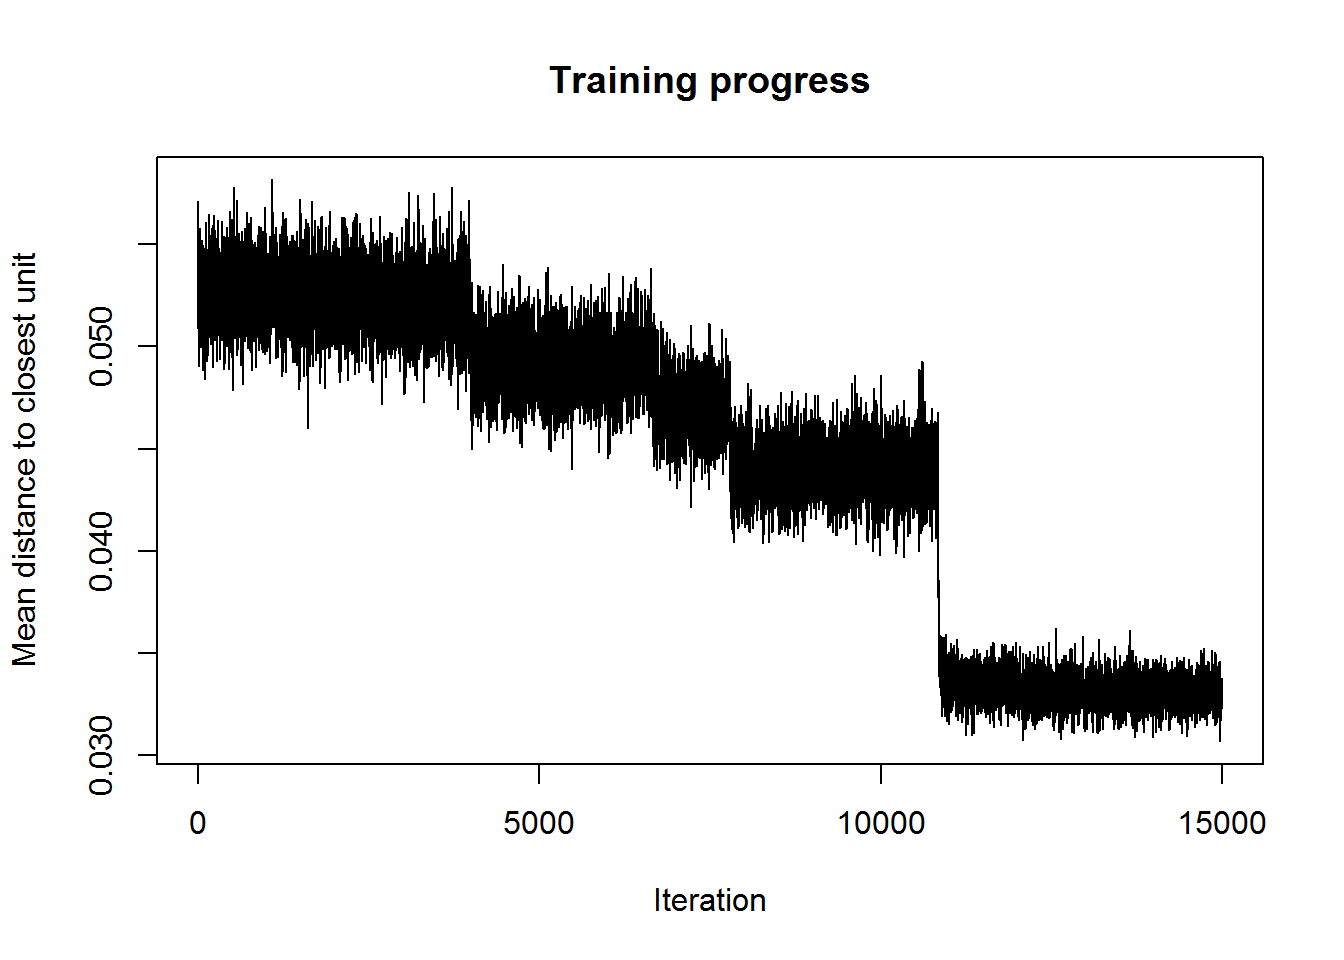
\includegraphics{bookdown-demo_files/figure-latex/unnamed-chunk-3-1.pdf}

\subsubsection{Node Counts}\label{node-counts}

This steps helps us visualize how many samples are mapped to each neuron
on the map. This can be used as an indicator of \textbf{map quality}.
Some key points:

\begin{itemize}
\tightlist
\item
  Sample distribution should be relatively uniform (colors or shades
  similar) throughout the map.
\item
  Large values in a map area are a sign that a larger map is needed.
\item
  Empty neurons are a sign that the map is to large.
\item
  It is costumary to aim for 5 to 10 samples per neuron for an ideal
  map.
\end{itemize}

\begin{Shaded}
\begin{Highlighting}[]
\KeywordTok{source}\NormalTok{(}\StringTok{'coolBlueHotRed.R'}\NormalTok{)}
\KeywordTok{plot}\NormalTok{(som_model,}
     \DataTypeTok{type =} \StringTok{"count"}\NormalTok{,}
     \DataTypeTok{palette.name =} \NormalTok{coolBlueHotRed,}
     \DataTypeTok{main =} \StringTok{"Counts plot / Map quality"}\NormalTok{)}
\end{Highlighting}
\end{Shaded}

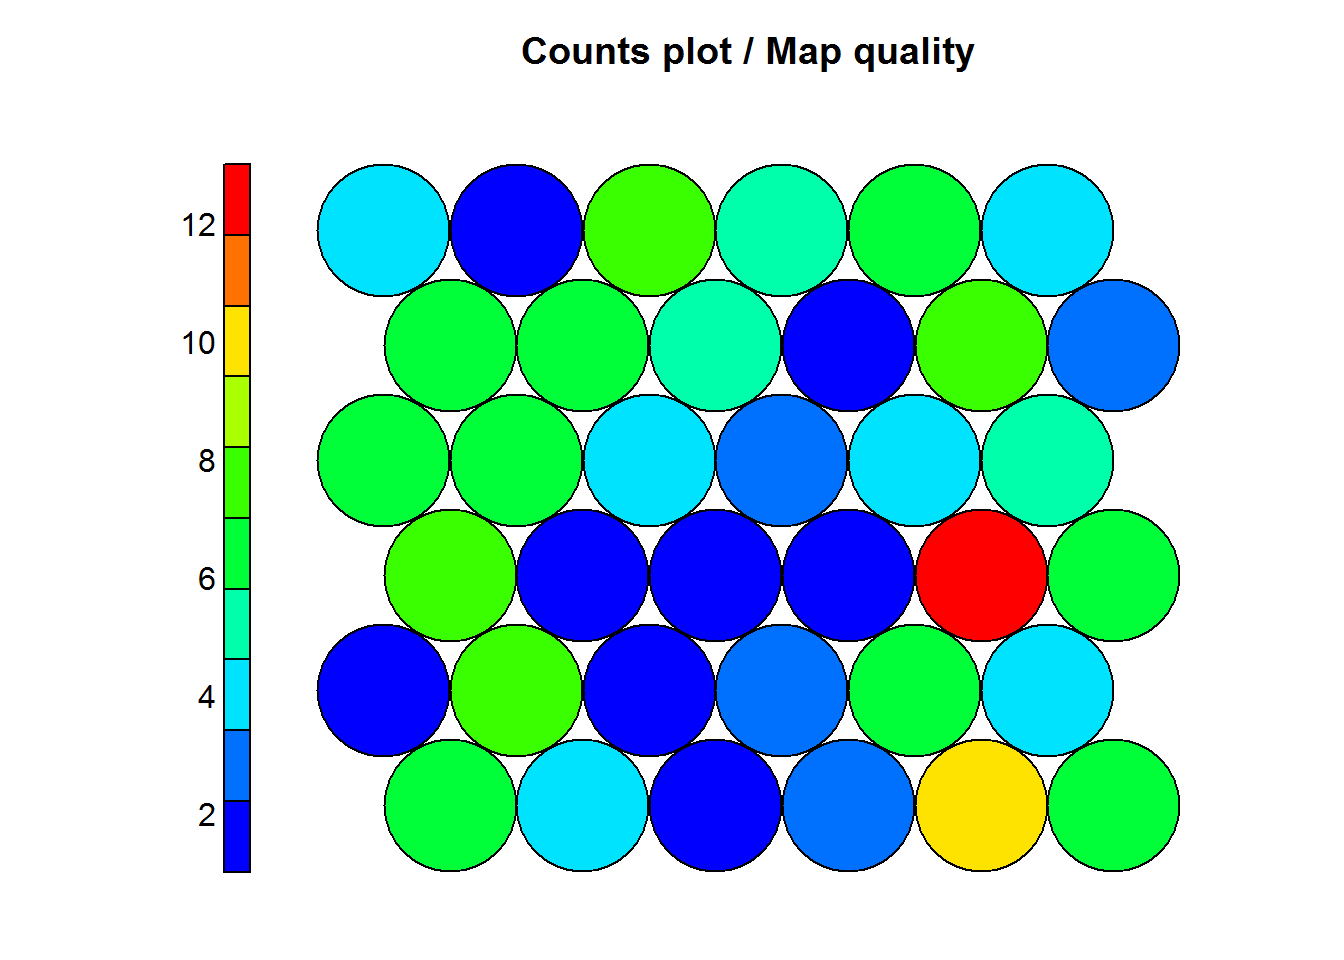
\includegraphics{bookdown-demo_files/figure-latex/unnamed-chunk-4-1.pdf}

\subsubsection{Neighbor Distance}\label{neighbor-distance}

This is also called the \textbf{\emph{U-Matrix}} and it is a
visualization of the distance between each neuron and it's neihgbors.
Key points:

\begin{itemize}
\tightlist
\item
  It's usually visualized using a grayscale.
\item
  Areas of low neighbor distance indicate groups of similar neurons.
\item
  Areas of high nighbor distance indicate that neurons are more
  dissimilar.
\item
  The U-Matrix can be used to identify clusters.
\end{itemize}

\begin{Shaded}
\begin{Highlighting}[]
\KeywordTok{plot}\NormalTok{(som_model,}
     \DataTypeTok{type =} \StringTok{"dist.neighbours"}\NormalTok{,}
     \DataTypeTok{palette.name =} \NormalTok{gray.colors,}
     \DataTypeTok{main =} \StringTok{"Nighbour distance plot/ U-Matrix"}\NormalTok{)}
\end{Highlighting}
\end{Shaded}

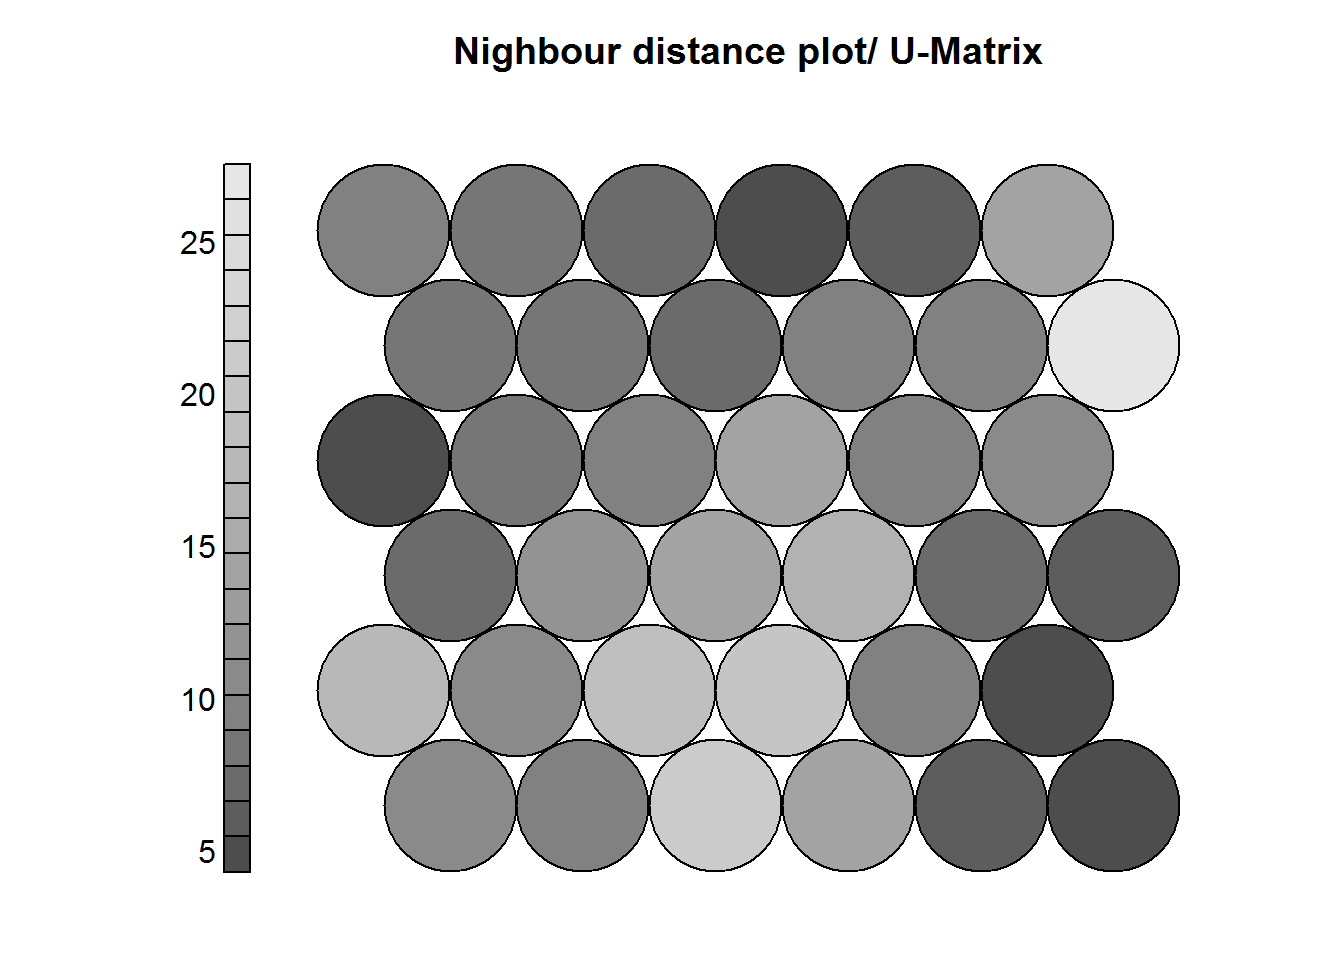
\includegraphics{bookdown-demo_files/figure-latex/unnamed-chunk-5-1.pdf}

\subsubsection{Weight vectors / Codes}\label{weight-vectors-codes}

These codes are made up of normalised values of the original variables
from the dataset used to train the SOM. Each node weight vector is
similar (representative) of the samples mapped to that node. By doing
this visualization it is possible to see patterns in the distribution of
the values of variables.

Key points:

\begin{itemize}
\tightlist
\item
  The visualization of \textgreater{}7 variables with this approach is
  usually of not much use.
\end{itemize}

\begin{Shaded}
\begin{Highlighting}[]
\KeywordTok{plot}\NormalTok{(som_model,}
     \DataTypeTok{type =} \StringTok{"codes"}\NormalTok{,}
     \DataTypeTok{main =} \StringTok{"Codes"}\NormalTok{,}
     \DataTypeTok{palette.name =} \NormalTok{coolBlueHotRed)}
\end{Highlighting}
\end{Shaded}

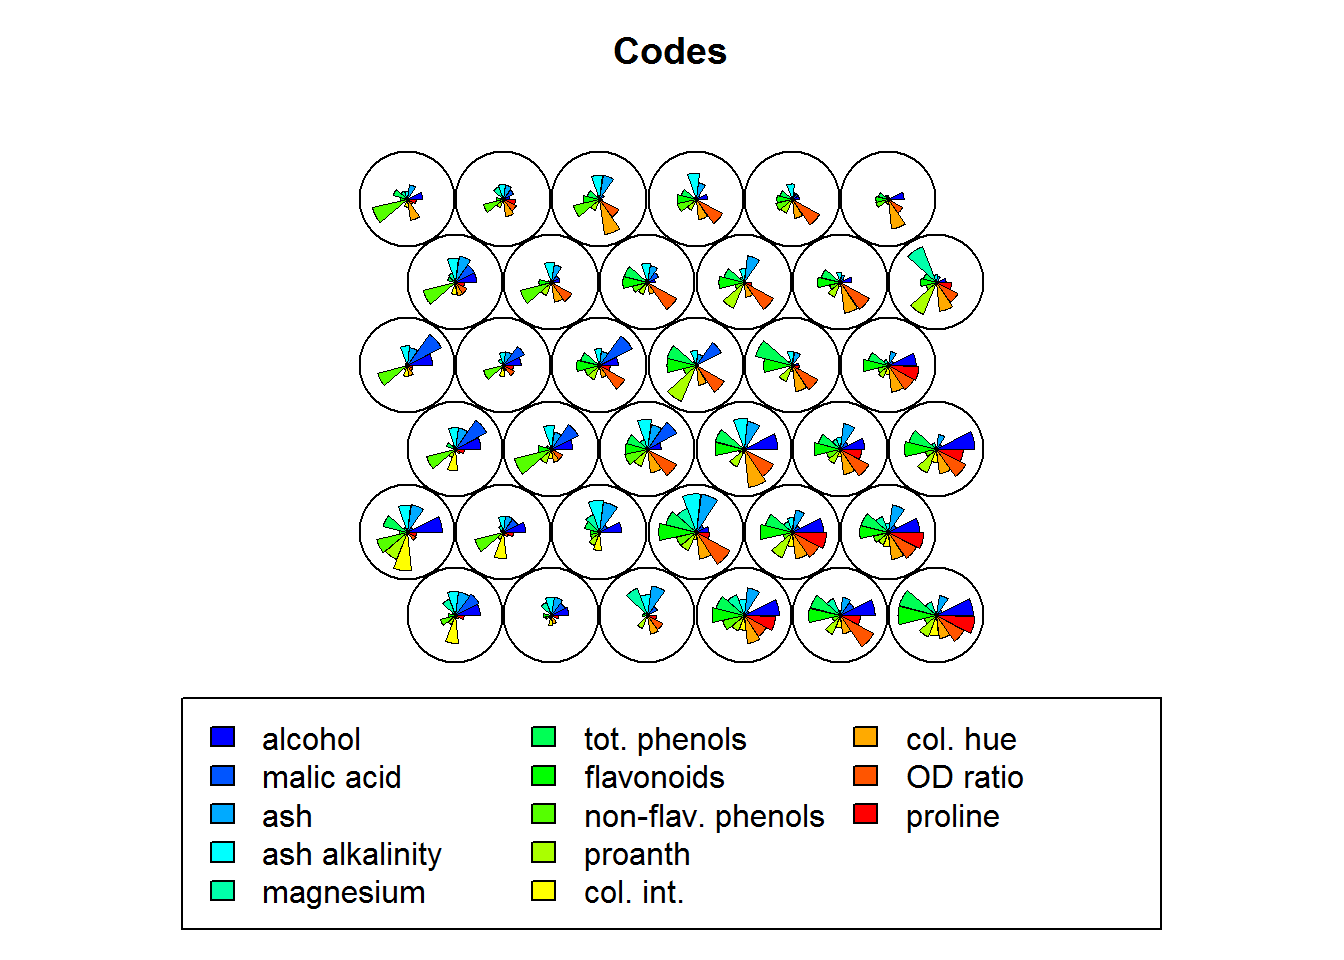
\includegraphics{bookdown-demo_files/figure-latex/unnamed-chunk-6-1.pdf}

\subsubsection{Heatmaps}\label{heatmaps}

One of the most important visualization of a SOM. It allows for a weight
space view of a single variable (distribution). Usually, multiple
heatmaps are produced based on different variables and then compared to
see if areas and/or patterns of interest are discovered. Key points:

\begin{itemize}
\tightlist
\item
  When generating multiple visualizations of the same SOM, individual
  sample positions do not move form one visualization to another, the
  map is simpleyu colored by different variables.
\end{itemize}

\begin{Shaded}
\begin{Highlighting}[]
\NormalTok{codes <-}\StringTok{ }\KeywordTok{as.data.frame}\NormalTok{(}\KeywordTok{as.list}\NormalTok{(som_model$codes))}

\CommentTok{#Standardized values}
\KeywordTok{plot}\NormalTok{(som_model,}
     \DataTypeTok{type =} \StringTok{"property"}\NormalTok{,}
     \DataTypeTok{property =} \NormalTok{codes$alcohol,}
     \DataTypeTok{palette.name =} \NormalTok{coolBlueHotRed,}
     \DataTypeTok{main =} \StringTok{"Standardized Alcohol Levels"}\NormalTok{)}
\end{Highlighting}
\end{Shaded}

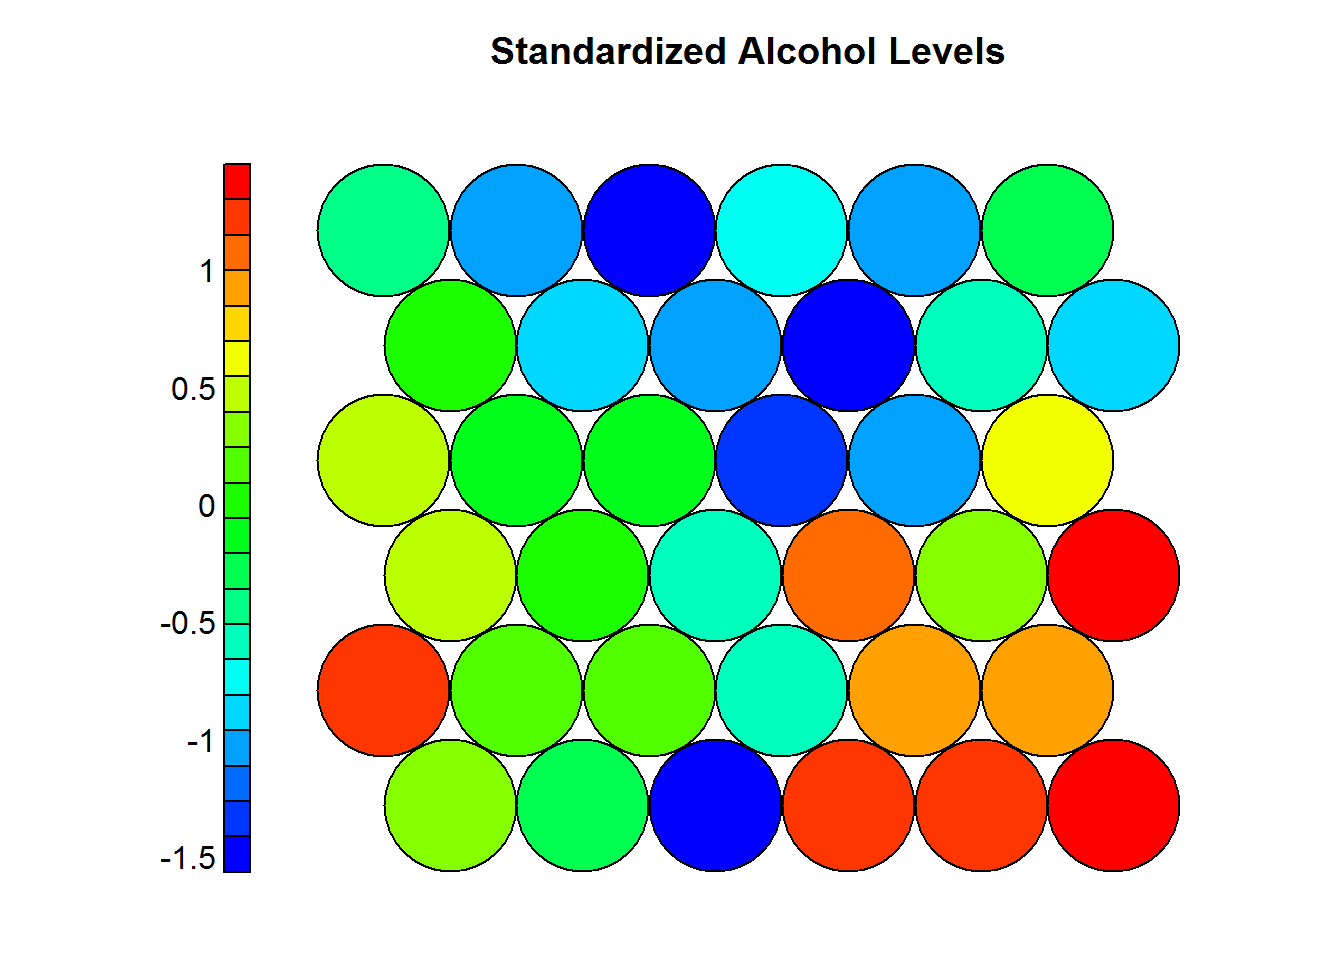
\includegraphics{bookdown-demo_files/figure-latex/unnamed-chunk-7-1.pdf}

Heat maps are usually presented to non-technicall people, therefore it
is prefered to use the normal values as they appeared on the original
dataset. The following heatmaps are presented with values previous to
standardization.

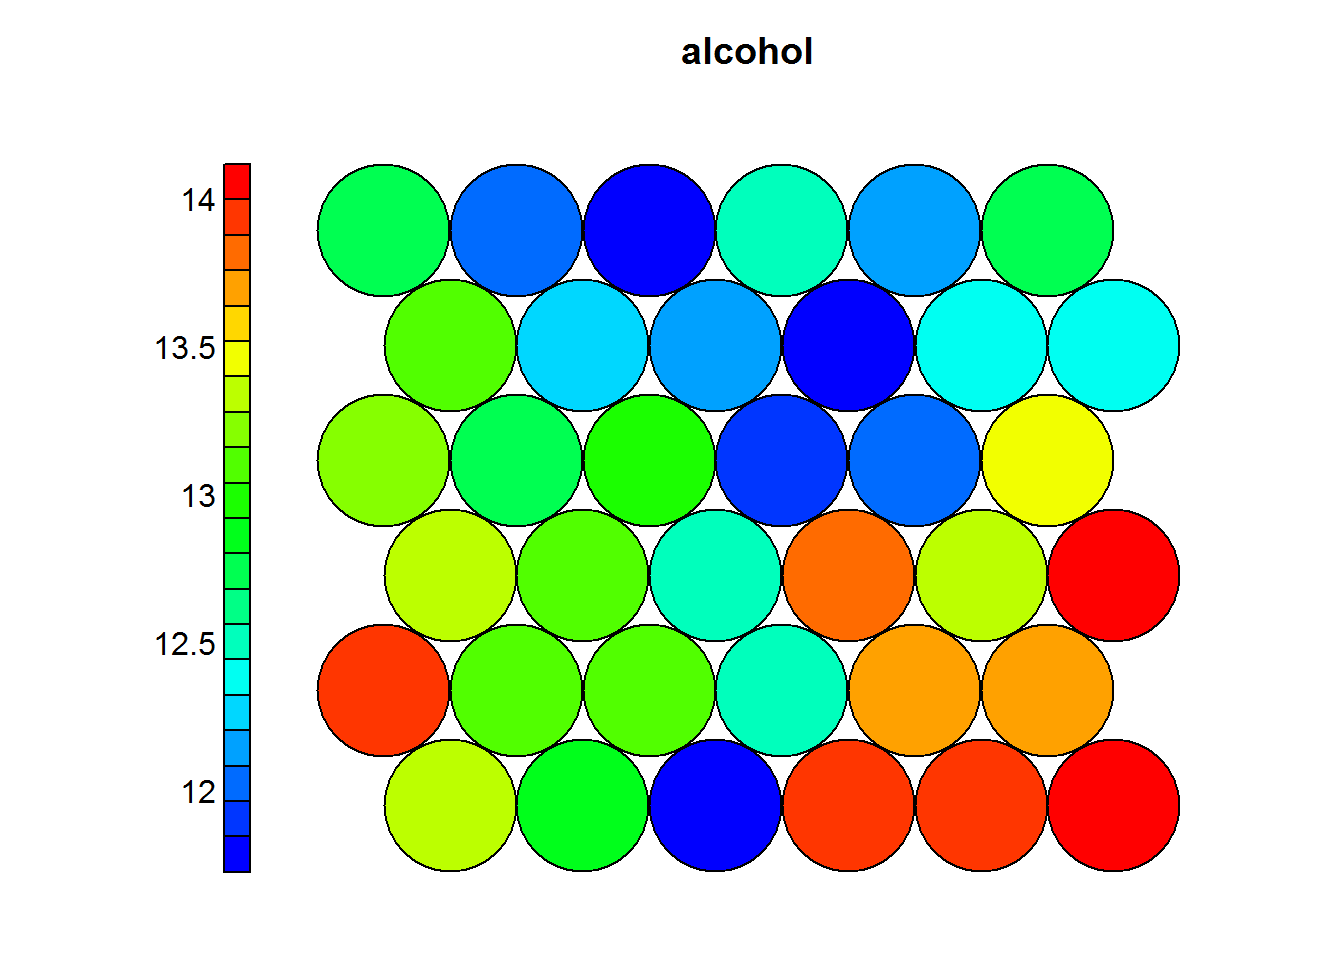
\includegraphics{bookdown-demo_files/figure-latex/unnamed-chunk-8-1.pdf}

\begin{figure}[htbp]
\centering
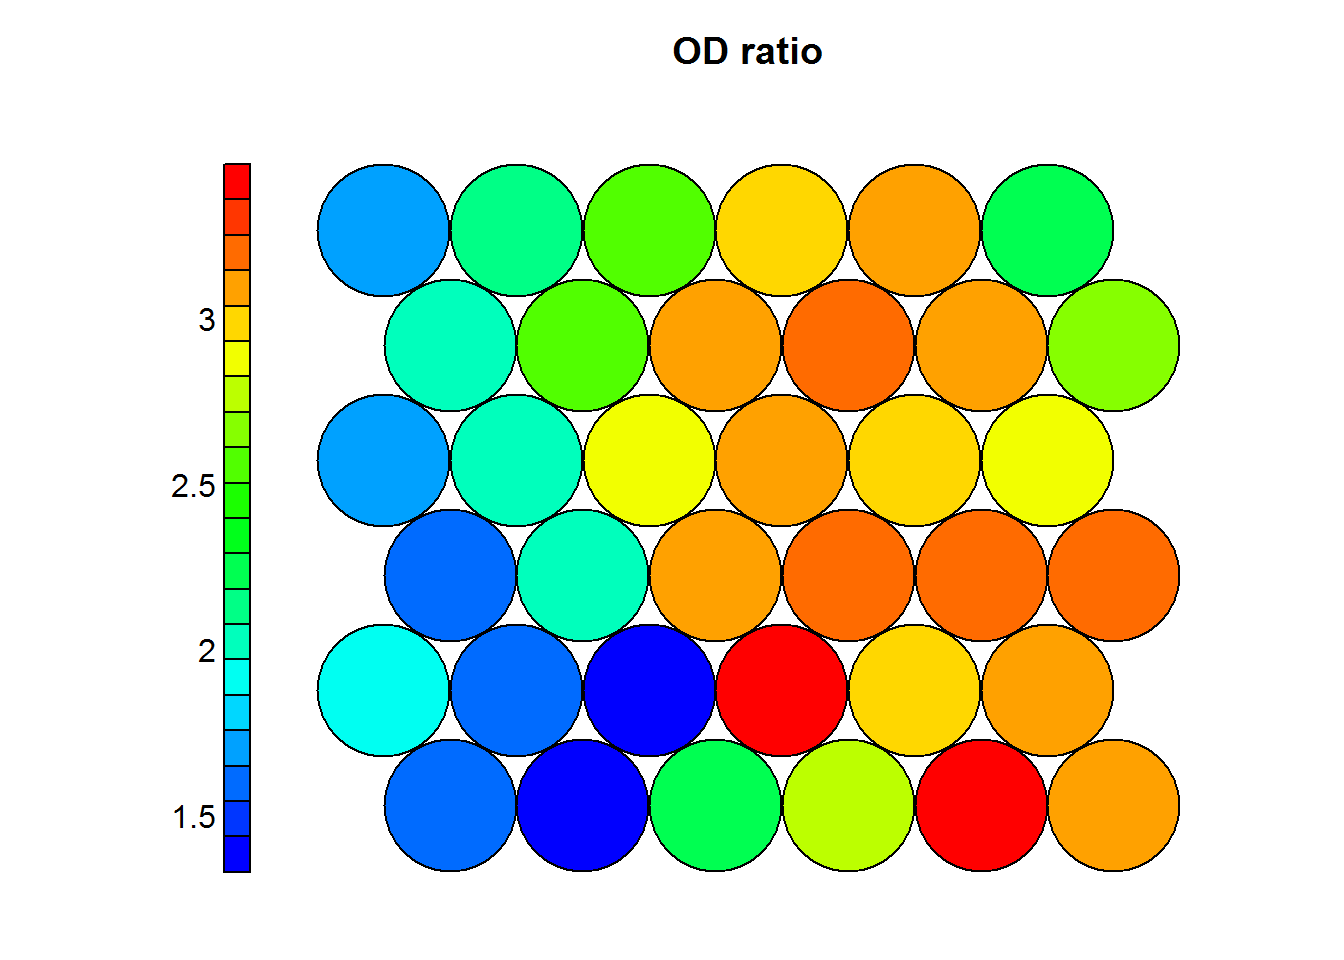
\includegraphics{bookdown-demo_files/figure-latex/unnamed-chunk-9-1.pdf}
\caption{\label{fig:unnamed-chunk-9}OD Ratio in Wines}
\end{figure}

\begin{figure}[htbp]
\centering
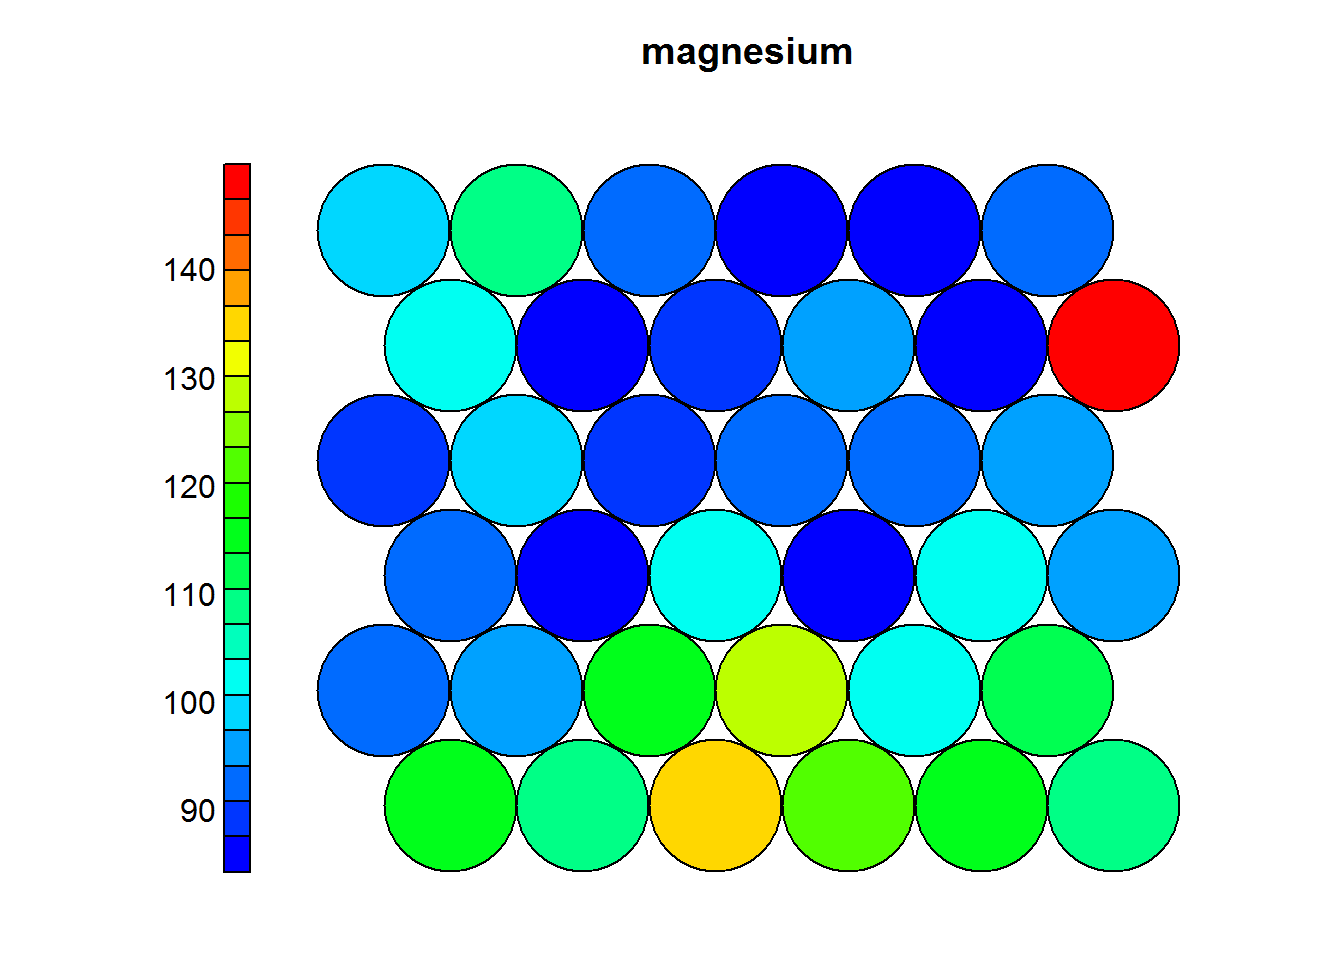
\includegraphics{bookdown-demo_files/figure-latex/unnamed-chunk-10-1.pdf}
\caption{\label{fig:unnamed-chunk-10}Magnesium levels in Wines}
\end{figure}

\begin{figure}[htbp]
\centering
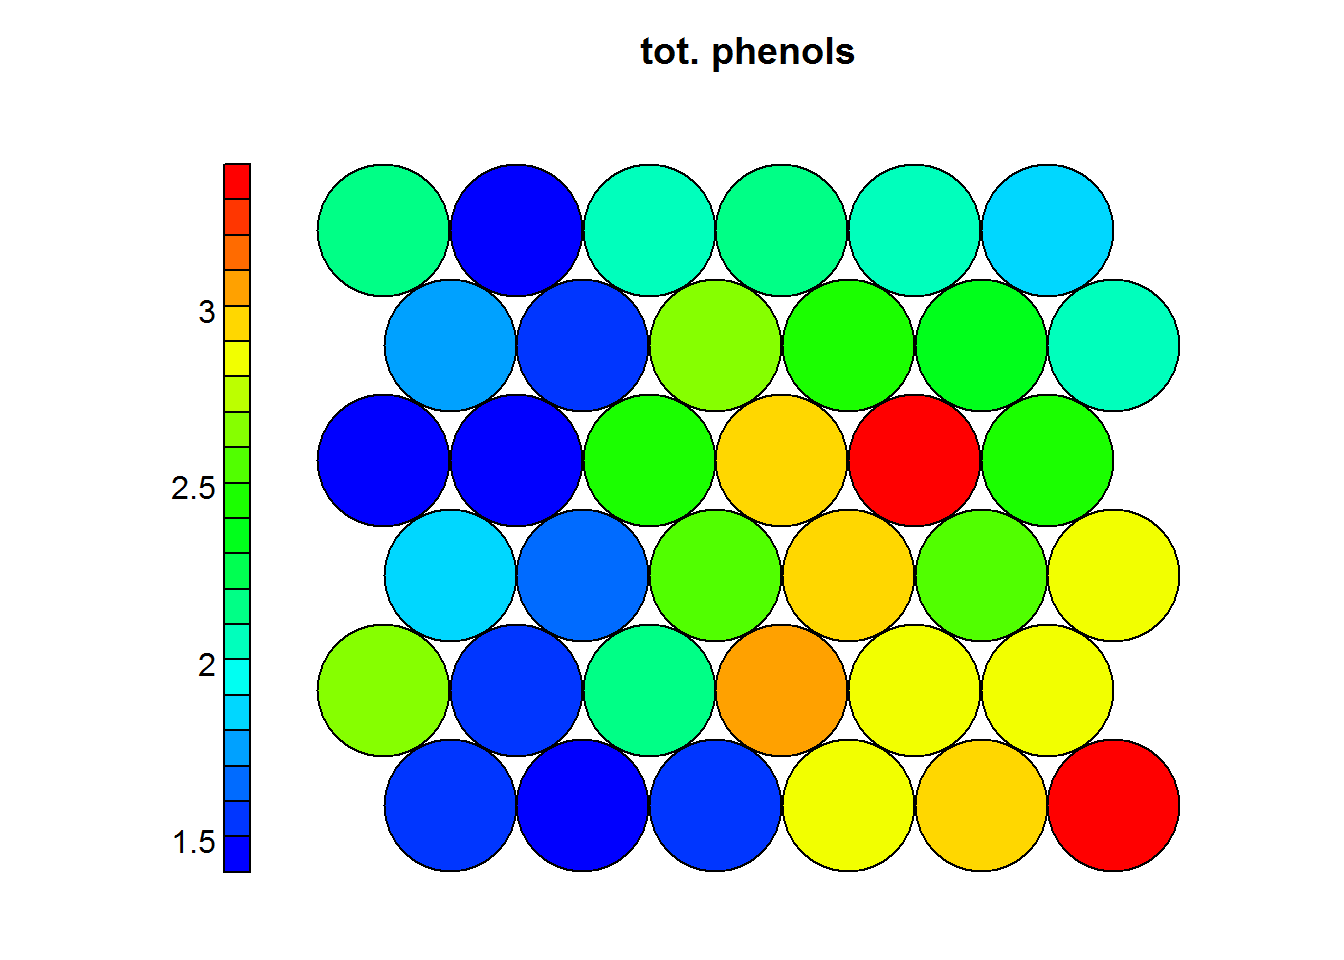
\includegraphics{bookdown-demo_files/figure-latex/unnamed-chunk-11-1.pdf}
\caption{\label{fig:unnamed-chunk-11}Total Phenols levels in Wines}
\end{figure}

\subsubsection{Drawing Conclusions}\label{drawing-conclusions}

Understanding how a Self Organizing Map is generated is of key value to
run these analysis. Once a clear understanding of the mathematics and
algorithmia is achieved then the process of training the SOM can start.
Special attention must be put in the quality of the SOM, the right
amount of ephocs and the size of the grid as well.

In the previous example one can see that wines with high levels of
alcohol tend to have low OD ratios and high levels of total phenols.
Combined with domain knowledge these assosiations can be put to good use
in the field.

\bibliography{packages,book}


\end{document}
